\newpage

\section{Partie 1: Quelques opérations de base sur les signaux}

\subsection{Signal numérique de synthèse}

\subsubsection{Génération du signal}

\begin{lstlisting}[language=python]
    def sinus_echant(f0, fe, N):
        t = np.arange(N) / fe
        signal = np.sin(2 * np.pi * f0 * t)

        plt.figure(figsize=(10, 4))
        plt.plot(t, signal)
        plt.title(f'Signal sinusoidal : f0 = {f0} Hz, fe = {fe} Hz, N = {N}')
        plt.xlabel('Temps (s)')
        plt.ylabel('Amplitude')
        plt.grid(True)
        plt.show()

    return signal
\end{lstlisting}


\begin{figure}[!h]
\begin{center}
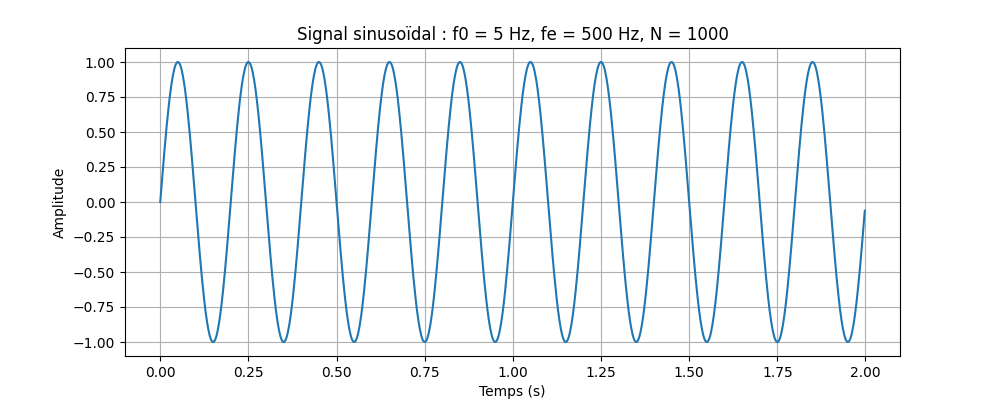
\includegraphics[width=17cm]{screenshots/signal_echantillone.png}
\end{center}
\caption{Signal sinusoïdal de fréquence f0 échantillonné à fe points
par seconde et comportant en tout N points}
\end{figure} 

\subsubsection{Energie et puissance}

Afin de calculer l'énergie et la puissance du signal sans utiliser de boucle for directement, on utilise:

\begin{lstlisting}[language=python]
    def energie_signal(signal):
        return np.sum(signal ** 2)

    def puissance_signal(signal):
        return np.mean(signal ** 2)
\end{lstlisting}

\begin{figure}[!h]
\begin{center}
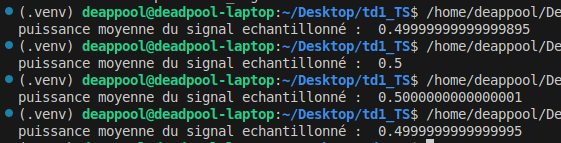
\includegraphics{screenshots/puissance_et_energie.png}
\end{center}
\caption{Comparaison entre la puissance moyenne théorique et la puissance moyenne calculée du signal}
\end{figure} 

\subsubsection{Quantification}

\begin{lstlisting}[language=python]
def quantifier(signal, N_bits):
    """Quantifie un signal sur N bits"""
    min_val, max_val = np.min(signal), np.max(signal)
    levels = 2 ** N_bits
    step = (max_val - min_val) / (levels - 1)
    quantized_signal = np.round((signal - min_val) / step) * step + min_val
    return quantized_signal
\end{lstlisting}

\begin{figure}[!h]
\begin{center}
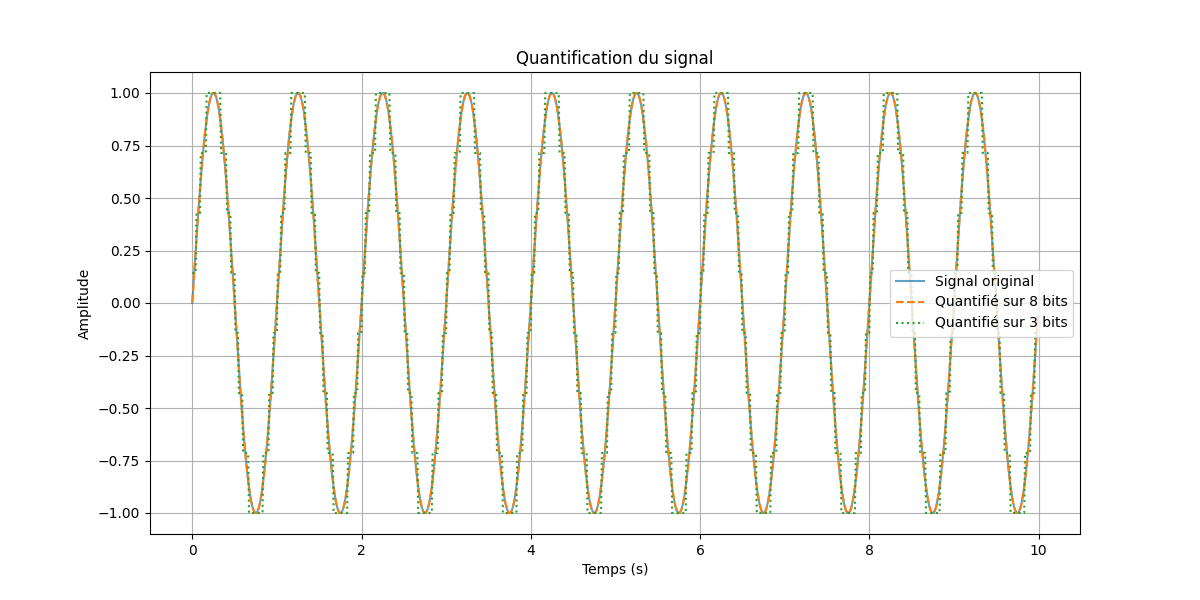
\includegraphics[width=17cm]{screenshots/Quantification.png}
\end{center}
\caption{Quantification du signal à 3 et 8 bits}
\end{figure} 

On remarque que le signal quantifié à 8 bits colle presque parfaitement à la courbe comparé au signal quantifié à 3 bits qui lui présente des paliers légérements visibles et qui donc colle moin au signal d'origine.\\ 

Ensuite on calcule SNR du signal pour les deux quantifications:

\begin{lstlisting}[language=python]
bruit_q8 = signal - signal_q8
bruit_q3 = signal - signal_q3

energie_bruit_q8 = energie_signal(bruit_q8)
energie_bruit_q3 = energie_signal(bruit_q3)

energie_signal = energie_signal(signal)

snr_q8 = 10 * np.log10(energie_signal / energie_bruit_q8) #en dB
snr_q3 = 10 * np.log10(energie_signal / energie_bruit_q3) #en dB
\end{lstlisting}

\begin{figure}[!h]
\begin{center}
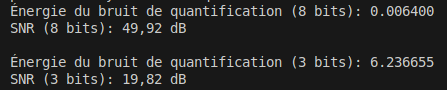
\includegraphics{screenshots/snr_quantification.png}
\end{center}
\caption{SNR pour chaque quantification}
\end{figure} 

On remarque que l'energie du bruit est plus élevée pour le signal quantifié à 3 bits. Le résultat est logique car on voit sur le graphe que ce signal est plus éloigné du signal d'origine comparé au signal quantifié à 8 bits. On a la méme conclusion en raisonant sur le SNR: $SNR_{q8} > SNR_{q3}$.

\subsection{Signal audio}

\subsubsection{Enregistrement}

Les deux mots enregistrés sont "Bonjour" et "ChatGpt".

\subsubsection{Restitution}

\begin{figure}[!h]
\begin{center}
\includegraphics[width=15cm]{screenshots/siganl_enregistré.png}
\end{center}
\caption{Signal enregistré avec Audacity}
\end{figure} 

On écoute ensuite le signal à des fréquences de restitution différentes : {fe}, {fe * 2} et {fe // 2}.\\

{\bf{Analyse du résultat:}}\\
\begin{itemize}
    \item {\bf{Durée:}} 
    \begin{itemize}
        \item Restituer à 2× fe → le son est plus rapide, la durée est divisée par 2.
        \item Restituer à 0.5× fe → le son est ralenti, la durée est doublée.
    \end{itemize}
    \item {\bf{Spectre:}} 
    \begin{itemize}
        \item À fréquence de restitution plus haute → son plus aigu (fréquences multipliées).
        \item À fréquence plus basse → son plus grave (fréquences divisées).
    \end{itemize}
\end{itemize}

\newpage
\subsubsection{Quantification}

{\bf{Analyse du résultat:}}
\begin{itemize}
    \item Moins de bits → moins de niveaux → plus d’erreurs d’arrondi → plus de bruit de quantification.
    \item À 3 bits, le signal est très "en escalier", ce qui altère fortement la qualité audio. L'audio est très bruité.
    \item À 8 bits, le son est encore reconnaissable, mais moins naturel. Cependant, il reste trés proche du signal enregistré qui lui est à 16 bits PCM.
\end{itemize}

\subsubsection{Extraction de mots}

Aprés avoir identifié l'intervalle de temps pour chaque mot dans le signal enregistré on utilise ce code pour séparer les deux mots:
\begin{lstlisting}[language=python]
n1 = int(0.3 * fe)     #0.3s 
n2   = int(2.3 * fe)   #2.3s 
n3 = int(4 * fe)       #4s 

mot1 = y[n1:n2]
mot2 = y[n2+1:n3]

print("Mot 1 :")
sd.play(mot1, fe)
sd.wait()

print("Mot 2 :")
sd.play(mot2, fe)
sd.wait()
\end{lstlisting}

\begin{figure}[h]
    \centering
    \begin{subfigure}[b]{0.45\textwidth}
        \centering
        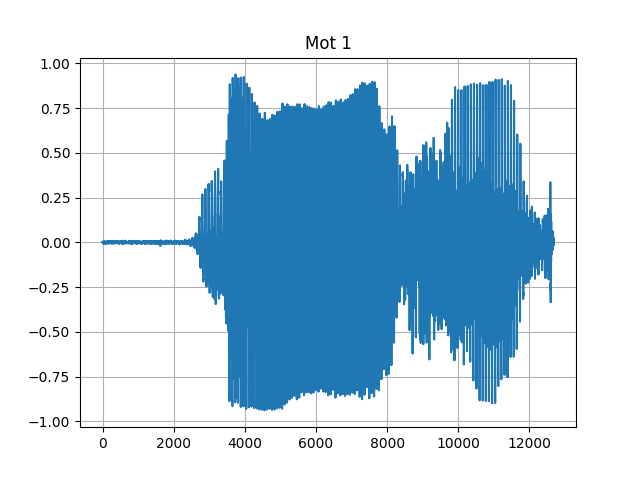
\includegraphics[width=9cm]{screenshots/mot1_graphe.png}
        \caption{Mot 1}
        \label{fig:mot1}
    \end{subfigure}
    \hfill
    \begin{subfigure}[b]{0.45\textwidth}
        \centering
        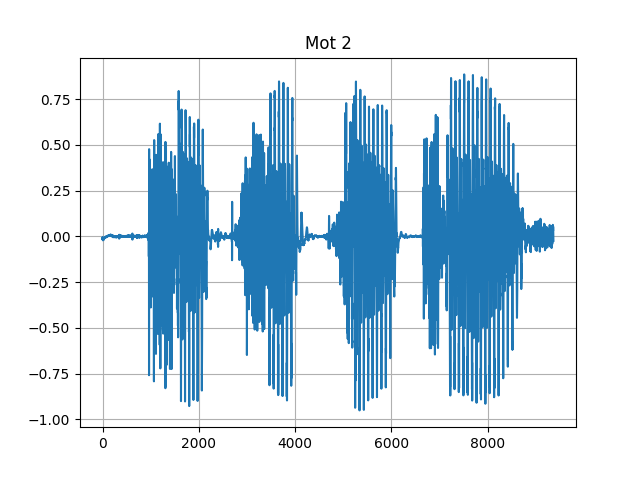
\includegraphics[width=9cm]{screenshots/mot2_graphe.png}
        \caption{Mot 2}
        \label{fig:mot2}
    \end{subfigure}
    \caption{Séparation des deux mots}
    \label{fig:Séparation des deux mots}
\end{figure}

Puis on enregistre les deux mots séparément dans des fichiers .wav :
\begin{lstlisting}[language=python]
    sf.write("mot1.wav", mot1, fe)
    sf.write("mot2.wav", mot2, fe)
\end{lstlisting}